\documentclass[../main.tex]{subfiles}
\begin{document}
\subsubsection{Modelling the shift}\label{subsubsec:modelling}

We will model the parameter shift $\Lambda(t)$ in such a way that the unstable equilibrium $x_{*}$ connects $x_{1}$ and $x_{2}$ in the past and forward limit respectively.
In this way we condition the basin of attraction $x_{2}$ to shrink from almost the entirity of the phase space $\Omega$ to almost only containing $x_{2}$ itself as time runs forward.
To do that we further reduce the dimensionality of our parameter space by letting $\alpha=1-\beta$.
This condition entails that $x_{*}=\beta$ which significantly simplifies our modelling procedure.
In fact now we can impose $\lambda(t):=\beta$ and choose an appropriate parameter shift $\Lambda(t)$ that satifies \eqref{eq:generic_shift}-\eqref{eq:generic_shift_derivative}.
This is done easily since $x_{*}\to x_{1/2}$, $t\to\pm\infty$ immediately translates in $\lambda_{-}=x_{1}=0$ and $\lambda_{+}=x_{2}=1$.
We can now pick any sigmoid function for $\Lambda(t)$ that connects $0$ to $1$ in $t\to\pm\infty$.
One choice is the hyperbolic tangent shift 

\begin{equation}\label{eq:tanh_shift}
     \Lambda(t) = \frac{1}{2}\big(\text{tanh}(\varepsilon t + \delta) + 1\big)\,, 
\end{equation}

which we parametrised in its ramp rate by $\varepsilon>0$ and its centering (in time) by $\delta\in \mathbb{R}$. 
Notice that by varying $\varepsilon$ we change the Lipschitz constant $L$ of $\Lambda(t)$ (essentially making the shift to ramp faster in the transient regime for larger values of $\varepsilon$) whereas by varying $\delta$ we change the subset $(t_{a}, t_{b})$ in \eqref{eq:generic_shift_derivative} when the transient regime occurs. 
Values $\varepsilon\to+\infty$ and $\delta\to0$ make the selected shift \eqref{eq:tanh_shift} to converge to the sign function. 

\begin{remark*}
     Any $C^{1}-$smooth, bounded function $f$ is Lipschitz with constant $L$ that coincides with $\sup\{|\newprime{f}(x_{j})|\}$, where $x_{j}\in\text{dom}\,f$ are stationary points of $\newprime{f}$.
\end{remark*}

\begin{figure}[H]
    \centering 
    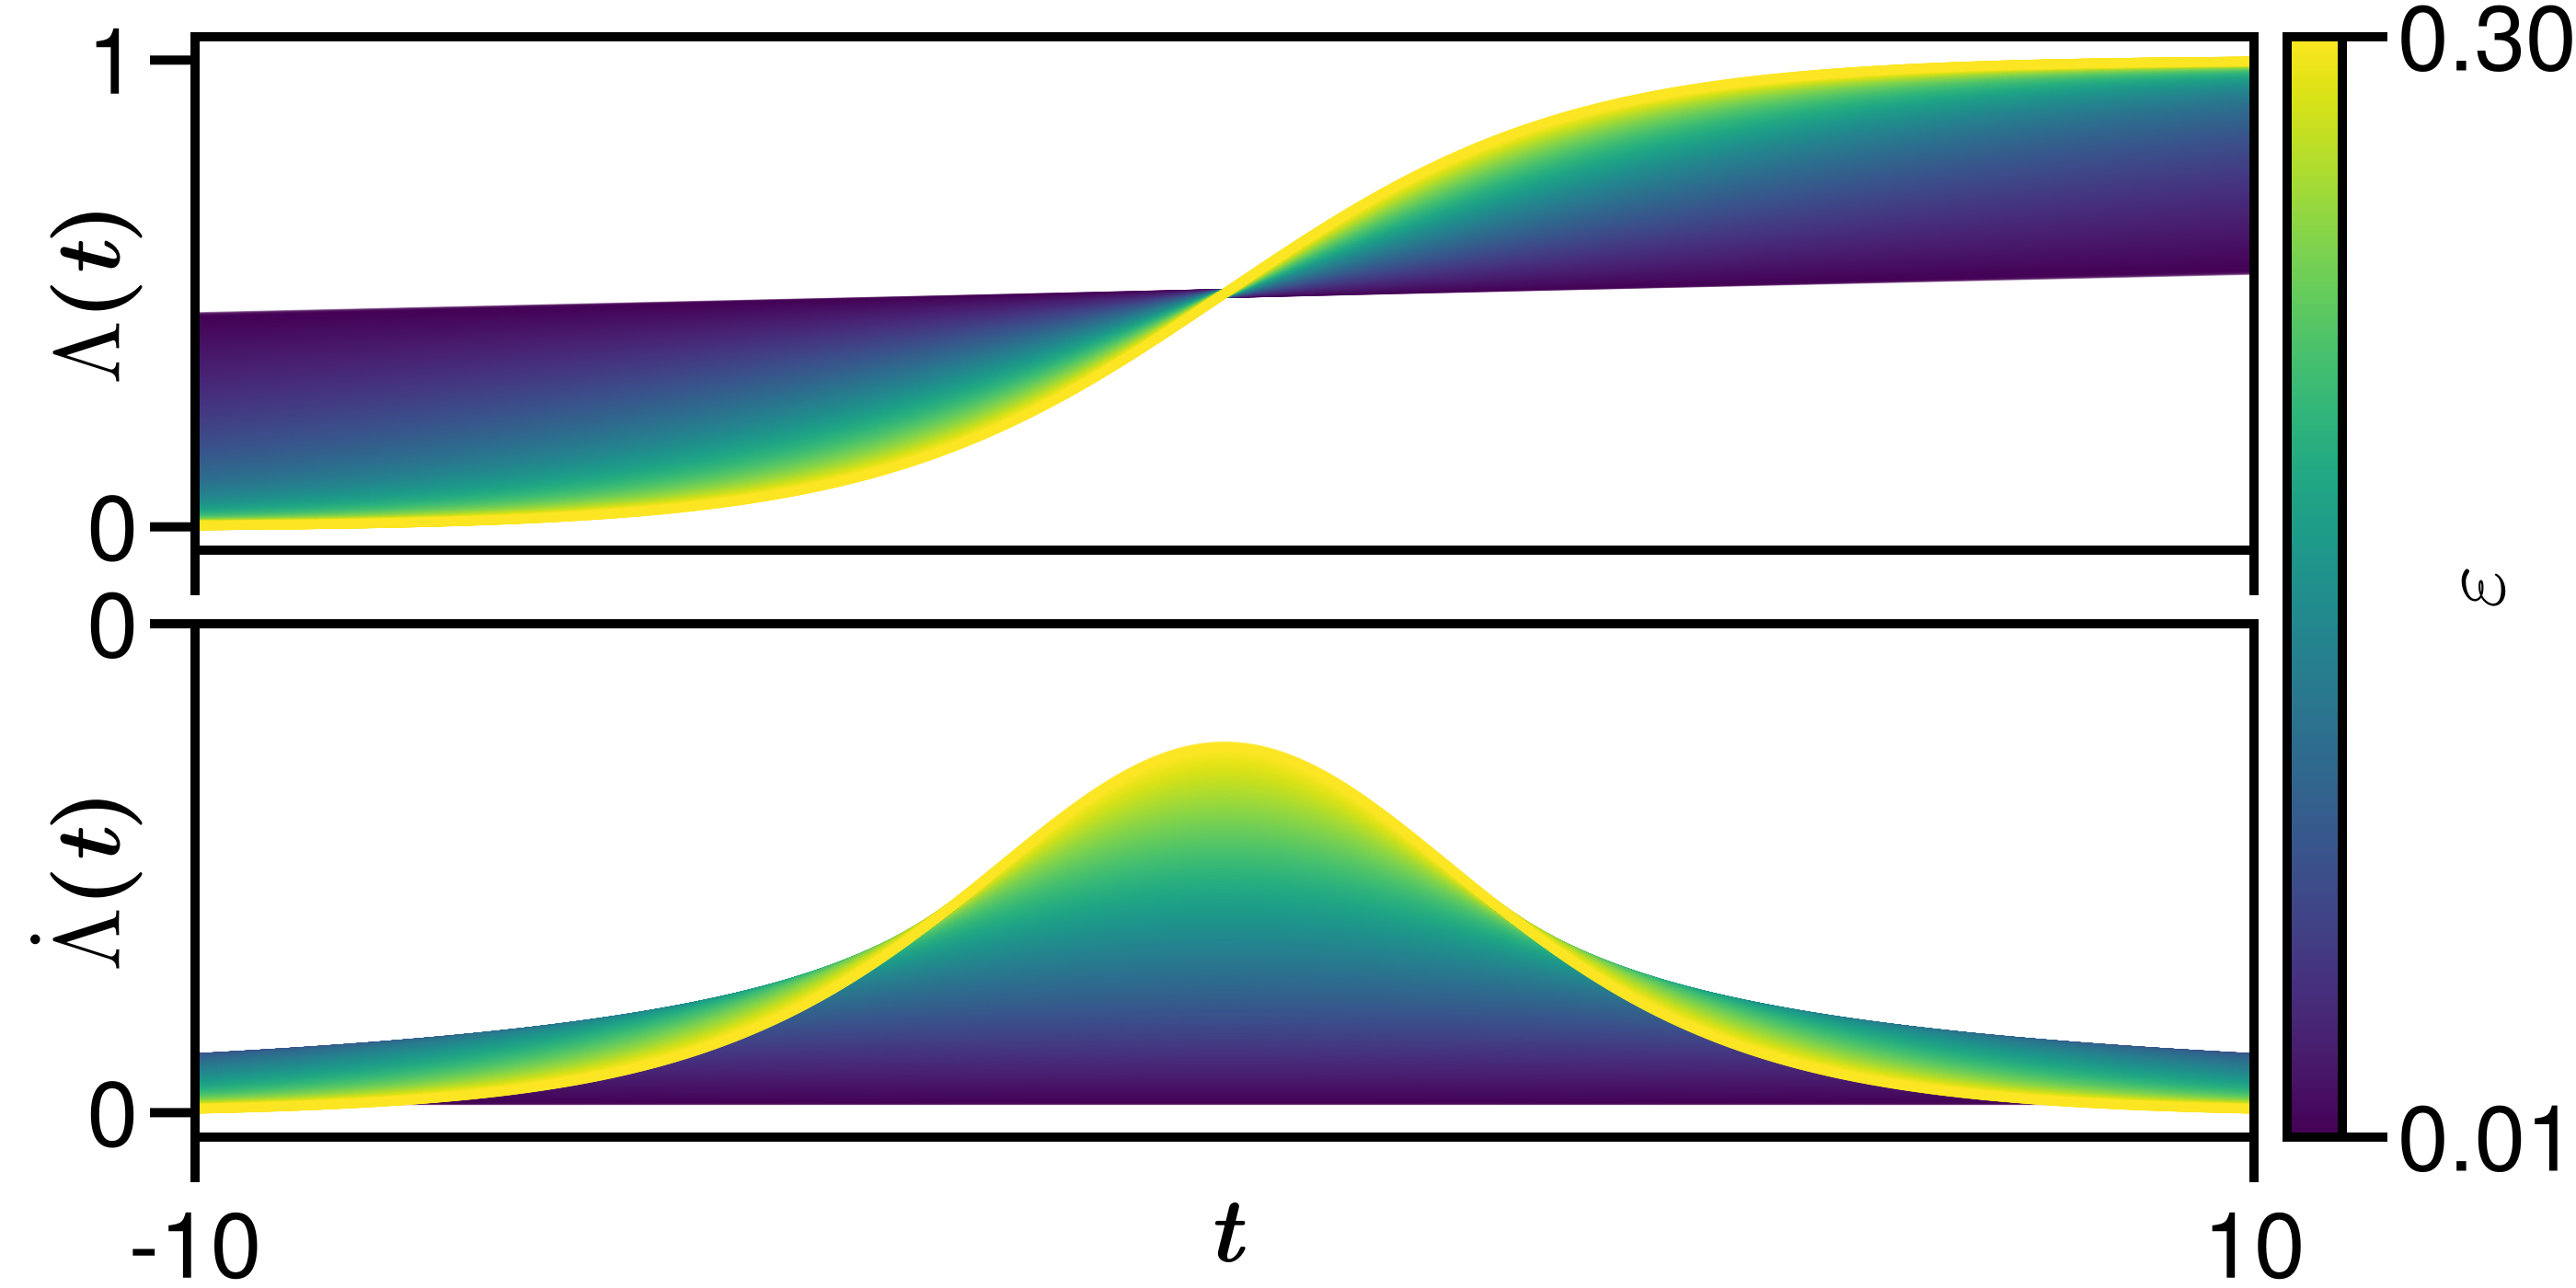
\includegraphics[keepaspectratio, width=\textwidth]{../figures/fig:sigmoid_example.png}
    \caption{Example of a sigmoid parameter shift $\Lambda(t) = $ (top) and its time derivative $\dot{\Lambda}(t) = $ (bottom). Different magnitudes of the shift's ramp $\varepsilon>0$ are color coded as per the colorbar on the left.
    }
    \label{fig:sigmoid_example}
\end{figure}

With the above we can formulate the non-autonomous augmented replicator system 

\begin{equation}\label{eq:nonautonomous_shifted_implicit}
   \begin{cases}
           \dot{x}(t) = x(1-x)(x - \lambda(t))\,, \\
           \dot{\lambda}(t) =  \frac{\varepsilon}{2}\,\text{sech}^{2}(\varepsilon t + \delta)\,,
   \end{cases}
\end{equation}

where $\dot{\lambda}(t) = \frac{d}{dt}\Lambda(t) = \dot{\Lambda}(t)$.

We would like to rewrite \eqref{eq:nonautonomous_shifted_implicit} so that it can be interpreted as a $2-$dimensional autonomous system.
To do that we drop the time dependence on $\lambda$ and $\dot{\lambda}$ and notice that
\begin{equation*}
        \text{tanh}(\varepsilon t + \delta) = 2\lambda - 1\quad \text{and}\quad \dot{\lambda} = \frac{\varepsilon}{2}\,\text{sech}^{2}(\varepsilon t + \delta) = \frac{\varepsilon}{2}\Big(1 - \text{tanh}^{2}(\varepsilon t + \delta)\Big) = \frac{\varepsilon}{2}\big(1 - (2\lambda - 1)^{2}\big)\,,
\end{equation*}

which, after trivial calculations, allows us to rewrite the non-autonomous system as

\begin{equation}\label{eq:nonautonomous_shifted}
   \begin{cases}
           \dot{x} = x(1-x)(x - \lambda(t))\,, \\
           \dot{\lambda} =  2\,\varepsilon\lambda(1-\lambda)\,.
   \end{cases}
\end{equation}

\end{document}
